\chapter{Estado del Arte}

\section{Sistemas ESD en la literatura}

En la literatura se han propuesto diversos sistemas relacionados con el control ESD.
Algunos trabajos se orientan al monitoreo continuo de la puesta a tierra mediante
tecnologías IoT, mientras que otros se enfocan en la detección de carga electrostática
en el cuerpo humano, circuitos integrados o tarjetas electrónicas. Sin embargo, las
propuestas identificadas no abordan de forma conjunta la verificación de pulseras
antiestáticas, identificación de usuario, almacenamiento local de registros, reportes e
interfaz de usuario en una estación de bajo costo para laboratorios de electrónica.

En el trabajo de Nagy \cite{Nagy2025} se propone un sistema de monitoreo continuo de
puesta a tierra mediante IoT. El sistema se compone de un servidor y módulos ubicados
en estaciones de trabajo. Estos módulos miden continuamente la resistencia del usuario
a tierra y la comparan con un umbral definido. En caso de que el umbral sea superado,
el sistema envía una alerta al servidor. El trabajo se centra principalmente en el diseño
de la tarjeta electrónica del servidor, sin extenderse al diseño detallado de los módulos
de medición instalados en las estaciones de trabajo. La Figura~\ref{fig:nagy2025_bloques}
muestra el diagrama general propuesto por el autor.

\begin{figure}[H]
    \centering
    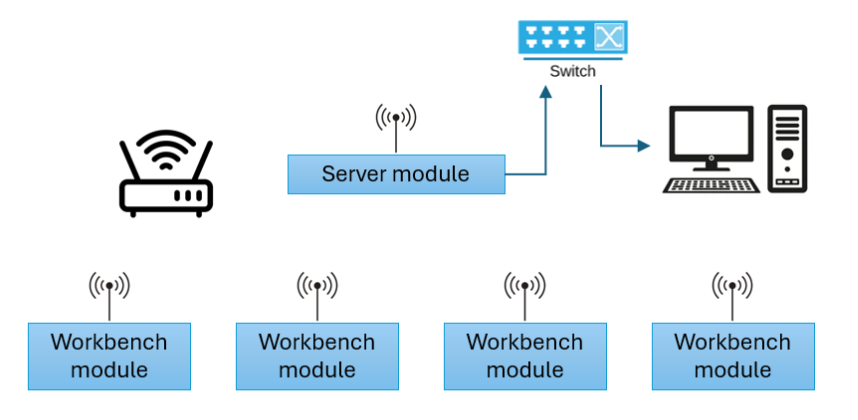
\includegraphics[width=0.8\textwidth]{pics/SA1_01.png}
    \caption{Diagrama de bloques del sistema propuesto por Nagy \cite{Nagy2025}.}
    \label{fig:nagy2025_bloques}
\end{figure}

La Figura~\ref{fig:nagy2025_servidor} presenta el diseño de la tarjeta electrónica
asociada al servidor del sistema.

\begin{figure}[H]
    \centering
    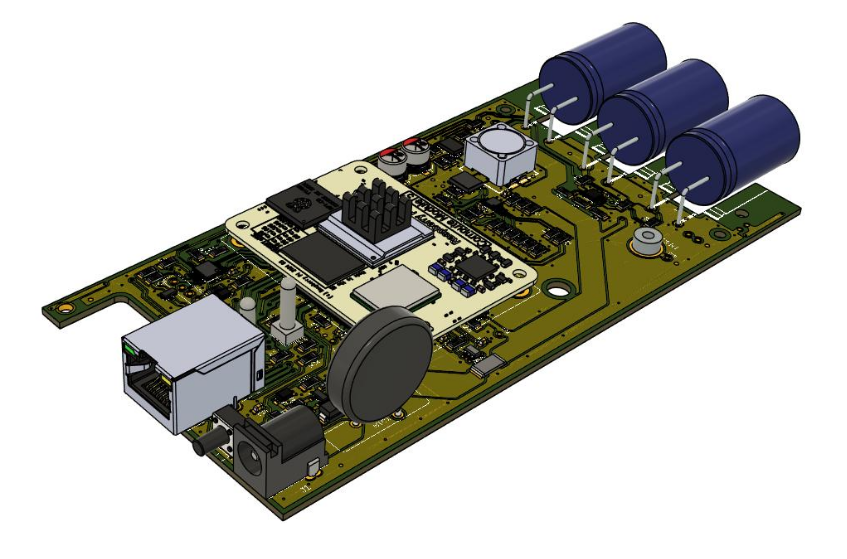
\includegraphics[width=0.8\textwidth]{pics/SA1_02.png}
    \caption{Diseño de la tarjeta electrónica para el servidor propuesto por Nagy
    \cite{Nagy2025}.}
    \label{fig:nagy2025_servidor}
\end{figure}

En el trabajo de Xu \cite{Xu2023} se diseña un sistema de medición de carga
electrostática en tarjetas electrónicas o líneas de producción de manufactura de
dispositivos electrónicos. La propuesta utiliza lectores de campo eléctrico instalados
en la línea de producción. Mediante motores y sistemas mecánicos, el sistema posiciona
el lector en puntos estratégicos de la línea, digitaliza las mediciones y las envía a un
servidor. La Figura~\ref{fig:xu2023_sistema} muestra el sistema propuesto.

\begin{figure}[H]
    \centering
    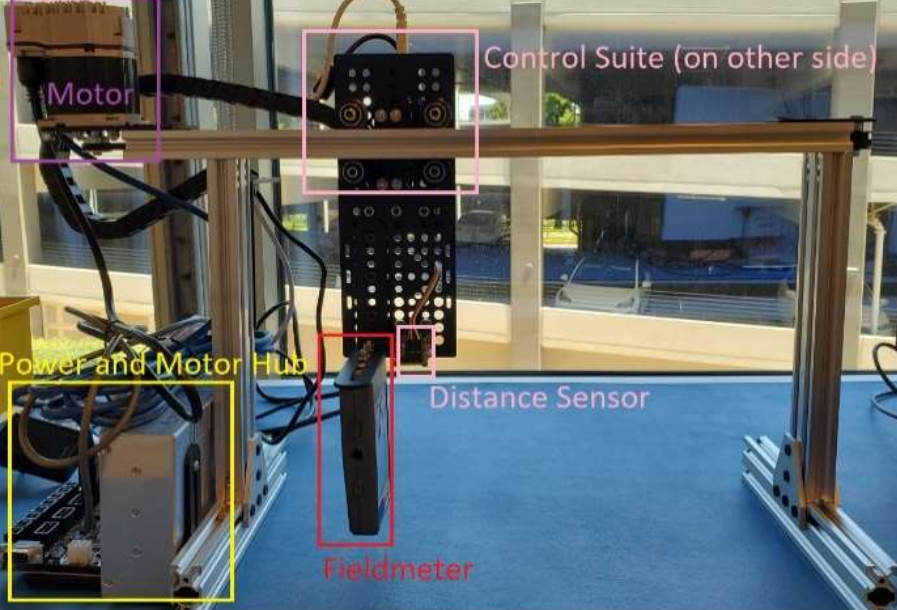
\includegraphics[width=0.8\textwidth]{pics/SA1_03.png}
    \caption{Sistema propuesto por Xu \cite{Xu2023}.}
    \label{fig:xu2023_sistema}
\end{figure}

Por otra parte, en el trabajo de Raúl \cite{URV2023} se automatiza una prueba de
ESD aplicada a dispositivos electrónicos automotrices. La prueba consiste en inyectar
una descarga electrostática al dispositivo bajo prueba y medir su respuesta. En dicho
trabajo, una prueba que anteriormente se realizaba de forma manual se automatiza
mediante el uso de un brazo robótico.

\section{Implementaciones de medición de resistencia en sistemas ESD}

El circuito electrónico principal en un sistema de control ESD es el encargado de medir
la resistencia del usuario a tierra. Actualmente, no se identifican circuitos integrados
tipo \textit{front-end} diseñados específicamente para esta aplicación, aunque la medición
de resistencia de alta impedancia es un tema ampliamente tratado en electrónica de
precisión. Además, los fabricantes de sistemas comerciales de control ESD usualmente no
publican los detalles de sus circuitos internos de medición. Por esta razón, resulta
necesario revisar alternativas disponibles para mediciones de impedancia y resistencia
en rangos elevados.

\vspace{2mm}

Una de las alternativas disponibles en el mercado es el AD5933 de Analog Devices,
un convertidor de impedancia con interfaz digital. Este dispositivo opera en un rango
aproximado de 1 k$\Omega$ a 10 M$\Omega$, utilizando señales alternas de estímulo con
frecuencias entre 1 kHz y 100 kHz \cite{AD5933}. Sin embargo, el AD5933 no está
orientado específicamente a la medición de resistencia de alta impedancia en DC. Esto
representa una limitación para la medición de resistencia cuerpo--tierra, ya que el valor
obtenido puede depender de la frecuencia de la señal de estímulo. La
Figura~\ref{fig:ad5933_bloques} muestra el diagrama de bloques de este dispositivo.

\begin{figure}[H]
    \centering
    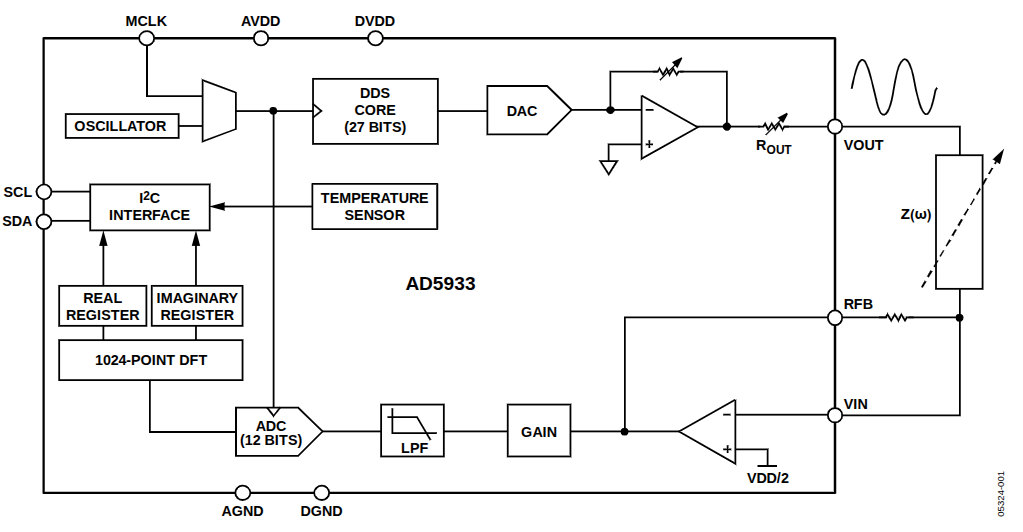
\includegraphics[width=0.6\textwidth]{pics/SA1_04.png}
    \caption{Diagrama de bloques del AD5933 \cite{AD5933}.}
    \label{fig:ad5933_bloques}
\end{figure}

También existen circuitos integrados como el ICL7106 de Analog Devices, perteneciente
a la categoría de circuitos para multímetros digitales. Este dispositivo corresponde a un
convertidor analógico-digital de 3.5 dígitos y permite implementar funciones de medición
de resistencia en instrumentos de bajo costo \cite{ICL7106}. No obstante, a diferencia
del AD5933, el ICL7106 no incorpora una interfaz de comunicación digital directa, lo que
dificulta su integración en un sistema inteligente de control ESD. Además, está diseñado
para operar con un display LCD, por lo que su uso en una arquitectura con
microcontrolador requeriría etapas adicionales de adaptación o lectura del display. La
Figura~\ref{fig:icl7106_operacion} muestra un circuito de operación típico.

\begin{figure}[H]
    \centering
    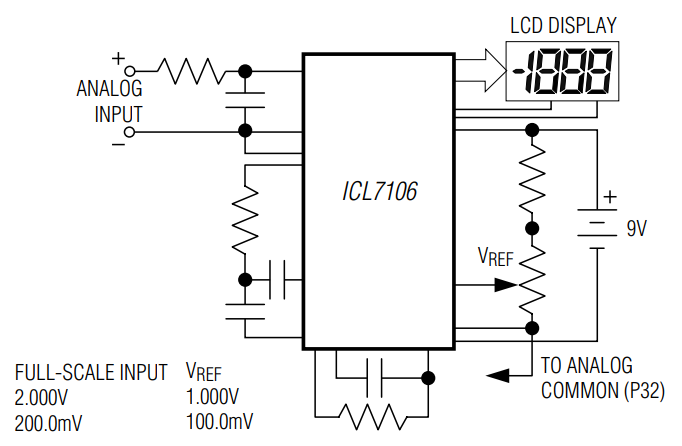
\includegraphics[width=0.6\textwidth]{pics/SA1_05.png}
    \caption{Circuito de operación típico del ICL7106 \cite{ICL7106}.}
    \label{fig:icl7106_operacion}
\end{figure}

Otras alternativas requieren el diseño de un circuito electrónico de precisión para medir
la resistencia cuerpo--tierra. Este tipo de medición involucra corrientes en el orden de
$\mu$A o nA, por lo que deben considerarse efectos como la corriente de polarización de
los amplificadores, las corrientes de fuga en la tarjeta electrónica, la contaminación
superficial, la humedad, el ruido eléctrico y la interferencia electromagnética. Por esta
razón, el diseño de un \textit{front-end} de medición para altas impedancias normalmente
requiere amplificadores operacionales de muy baja corriente de polarización, técnicas de
guardado (\textit{guarding}), blindaje, filtrado y criterios de diseño de PCB orientados a
reducir corrientes parásitas \cite{keithley_lowlevel}. Por estas razones, el diseño de un
circuito propio de medición de alta impedancia no se incorpora en la solución propuesta y
se utiliza un probador comercial como subsistema de verificación ESD.

\section{Normativas aplicables a sistemas ESD}

Los estándares aplicables a sistemas de control ESD se relacionan principalmente con
programas de control electrostático, puesta a tierra del personal, métodos de medición y
seguridad eléctrica del usuario. La Tabla~\ref{tab:esd_normas} resume las normativas más
relevantes para el contexto del proyecto.

\begin{table}[H]
\centering
\caption{Principales normativas aplicables a sistemas de control ESD.}
\label{tab:esd_normas}
\begin{tabular}{|l|p{10cm}|}
\hline
\textbf{Norma} & \textbf{Descripción} \\
\hline
ANSI/ESD S20.20 &
Establece los requisitos para implementar un programa de control ESD en entornos
industriales. Define procedimientos para la puesta a tierra del personal, control de
materiales y verificación de cumplimiento \cite{ANSI_S2020_Blog}. \\
\hline
IEC 61340-5-1 &
Norma internacional que especifica requisitos generales para la protección contra
descargas electrostáticas en áreas protegidas (EPA) \cite{IEC61340_Preview}. \\
\hline
ANSI/ESD STM97.1 &
Define el método de medición de la resistencia del sistema persona-calzado-suelo,
utilizado para evaluar la efectividad de la puesta a tierra del operador mediante calzado
ESD \cite{STM97_ANSI}. \\
\hline
ANSI/ESD S1.1 &
Establece el método de prueba para pulseras antiestáticas (\textit{wrist straps}),
incluyendo criterios de verificación de resistencia para favorecer una disipación adecuada
de carga \cite{S1_1_ANSI}. \\
\hline
IEC 61000-4-2 &
Describe el método de ensayo de inmunidad a descargas electrostáticas a nivel de sistema,
simulando eventos ESD para evaluar la robustez de equipos electrónicos
\cite{IEC61000_ITU}. \\
\hline
JEDEC JS-001 &
Define el modelo de descarga del cuerpo humano (HBM) para caracterizar la susceptibilidad
ESD de dispositivos semiconductores a nivel de componente \cite{JEDEC_JTR001}. \\
\hline
IEC 60479 &
Define efectos de la corriente eléctrica sobre el cuerpo humano, lo que permite considerar
límites de corriente y tensión para que el sistema sea seguro para el usuario
\cite{IEC60479_Resume}. \\
\hline
IEC 60601-1 &
Es una norma para dispositivos médicos principalmente, define criterios de 
seguridad para dispositivos eléctricos que realizen una conexión eléctrica con una persona \cite{iec60601_1}. \\
\hline
\end{tabular}
\end{table}

De las normativas mencionadas, las más relevantes para el diseño de un sistema de control
ESD en laboratorios de electrónica son ANSI/ESD S20.20, IEC 61340-5-1, ANSI/ESD
STM97.1, ANSI/ESD S1.1 e IEC 60479. Estas normas establecen requisitos asociados a la
puesta a tierra del personal, control de materiales, verificación de cumplimiento, métodos
de medición de resistencia y seguridad del usuario. Una limitación importante es que
varias de estas normativas no se encuentran disponibles gratuitamente, por lo que en este
documento se utilizan resúmenes, extractos, documentos de vista previa y material técnico
publicado por organizaciones relacionadas con el control ESD que hacen referencia a estas
normas.

\vspace{2mm}

En términos generales, los sistemas de puesta a tierra del personal deben mantener la
resistencia dentro de rangos que permitan disipar carga electrostática de forma controlada,
sin exponer al usuario a corrientes peligrosas. Para aplicaciones de control ESD, valores
de referencia como 750 k$\Omega$ y 35 M$\Omega$ son utilizados comúnmente en la evaluación
de sistemas de puesta a tierra del personal \cite{IEC61340_Preview}. Además, la
seguridad eléctrica del usuario debe considerarse de acuerdo con los límites de corriente
aplicables al cuerpo humano \cite{IEC60479_Resume}.

\section{Sistemas comerciales de control ESD}

Actualmente existen diversos sistemas comerciales de control ESD, desde dispositivos
económicos para verificar el funcionamiento de pulseras antiestáticas hasta estaciones
inteligentes diseñadas para controlar el ingreso a áreas de manufactura electrónica. Estas
soluciones permiten identificar diferentes niveles de funcionalidad, costo e integración.

Desco Industries ofrece el producto Desco 19240, un probador de pulseras antiestáticas
con indicación local de resultado. Este dispositivo tiene un costo aproximado de 150 USD
\cite{Desco_19240} y se limita a indicar estados como \textit{Pass}, \textit{Fail} u
\textit{Open}, dependiendo de la resistencia medida. Sin embargo, no incorpora capacidad
de comunicación digital, lo cual dificulta su integración directa en un sistema inteligente
de control ESD. La Figura~\ref{fig:desco19240_tester} muestra este equipo.

\begin{figure}[H]
    \centering
    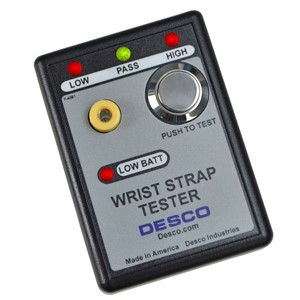
\includegraphics[width=0.4\textwidth]{pics/SAL4_01.jpg}
    \caption{Probador de pulseras antiestáticas Desco 19240 \cite{Desco_19240}.}
    \label{fig:desco19240_tester}
\end{figure}

La empresa SCS, parte de Desco Industries, ofrece el producto 770758 Dual Combination
Wrist Strap and Footwear Tester. Este equipo permite verificar simultáneamente la
resistencia de pulseras antiestáticas y calzado ESD. Su costo aproximado es de 1181 USD
\cite{SCS_770758}. Al igual que otros probadores básicos, su operación se basa
principalmente en indicaciones locales de aprobación o rechazo, sin capacidad de
comunicación digital para registro automático de eventos. La
Figura~\ref{fig:scs770758_tester} muestra este dispositivo.

\begin{figure}[H]
    \centering
    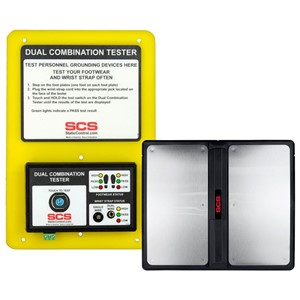
\includegraphics[width=0.4\textwidth]{pics/SAL4_02.jpg}
    \caption{Probador SCS 770758 para pulsera antiestática y calzado ESD
    \cite{SCS_770758}.}
    \label{fig:scs770758_tester}
\end{figure}

Transforming Technologies ofrece el producto PGT120 Combination ESD Tester for
Personal Grounding Equipment, con un costo aproximado de 2137 USD \cite{PGT120}. Este
dispositivo es similar al SCS 770758 en cuanto a la verificación de elementos de puesta a
tierra del personal, pero además puede utilizarse para habilitar mecanismos de control de
acceso, como puertas o barreras. La misma empresa ofrece el modelo PGT130.DT, el cual
incorpora lectura RFID y generación de reportes, con un costo aproximado de 7676 USD
\cite{PGT130DT}. Ambos equipos se muestran en la Figura~\ref{fig:pgt_modelos}.

\begin{figure}[H]
\centering

\begin{subfigure}[t]{0.45\textwidth}
    \centering
    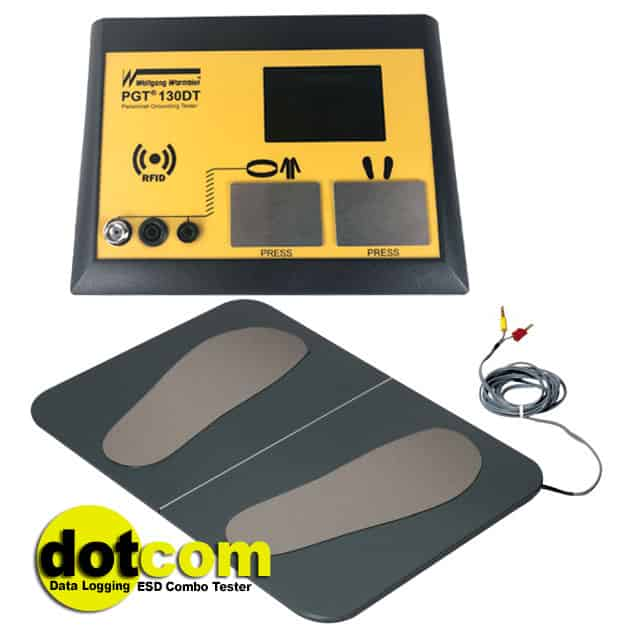
\includegraphics[width=\textwidth]{pics/SAL4_03.jpg}
    \caption{PGT130.DT \cite{PGT130DT}.}
    \label{fig:pgt130dt}
\end{subfigure}
\hfill
\begin{subfigure}[t]{0.45\textwidth}
    \centering
    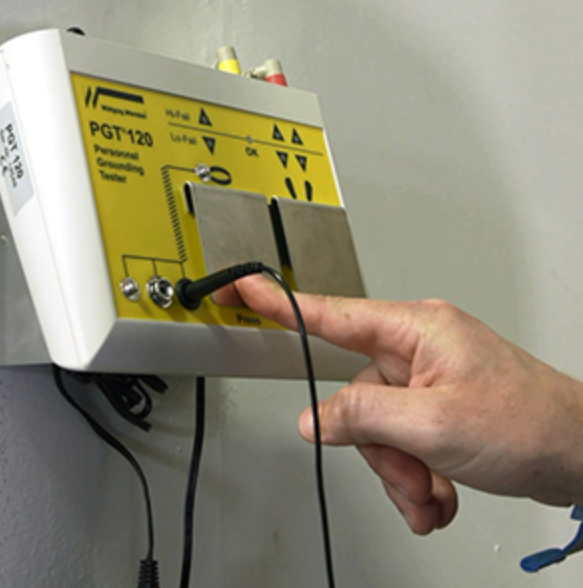
\includegraphics[width=\textwidth]{pics/SAL4_04.png}
    \caption{PGT120 \cite{PGT120}.}
    \label{fig:pgt120}
\end{subfigure}

\caption{Modelos PGT de Transforming Technologies.}
\label{fig:pgt_modelos}
\end{figure}

Finalmente, existen sistemas inteligentes de control ESD, como el ESDMAN ESD Access
Control System y el SmartLog Pro 2 de Desco Industries. El sistema ESDMAN tiene un
costo aproximado de 2500 USD en su versión básica \cite{ESDMAN_0016809}, mientras
que el SmartLog Pro 2 presenta un precio inicial cercano a 5643 USD \cite{SmartLogPro2}.
Ambos sistemas integran verificación de pulsera y calzado, identificación de usuario,
generación de reportes y control de acceso mediante comunicación de red. La
Figura~\ref{fig:sistemas_esd_avanzados} muestra ejemplos de este tipo de soluciones.

\begin{figure}[H]
\centering

\begin{subfigure}[t]{0.45\textwidth}
    \centering
    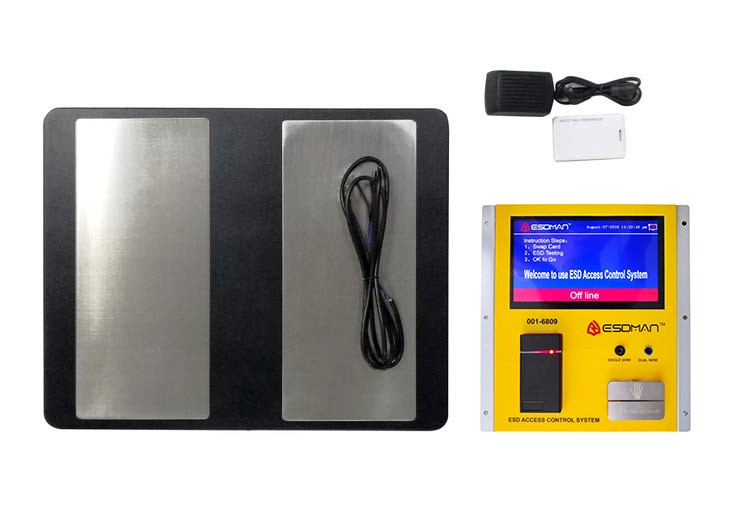
\includegraphics[width=\textwidth]{pics/SAL4_05.jpg}
    \caption{ESDMAN Access Control System \cite{ESDMAN_0016809}.}
    \label{fig:esdman_access}
\end{subfigure}
\hfill
\begin{subfigure}[t]{0.45\textwidth}
    \centering
    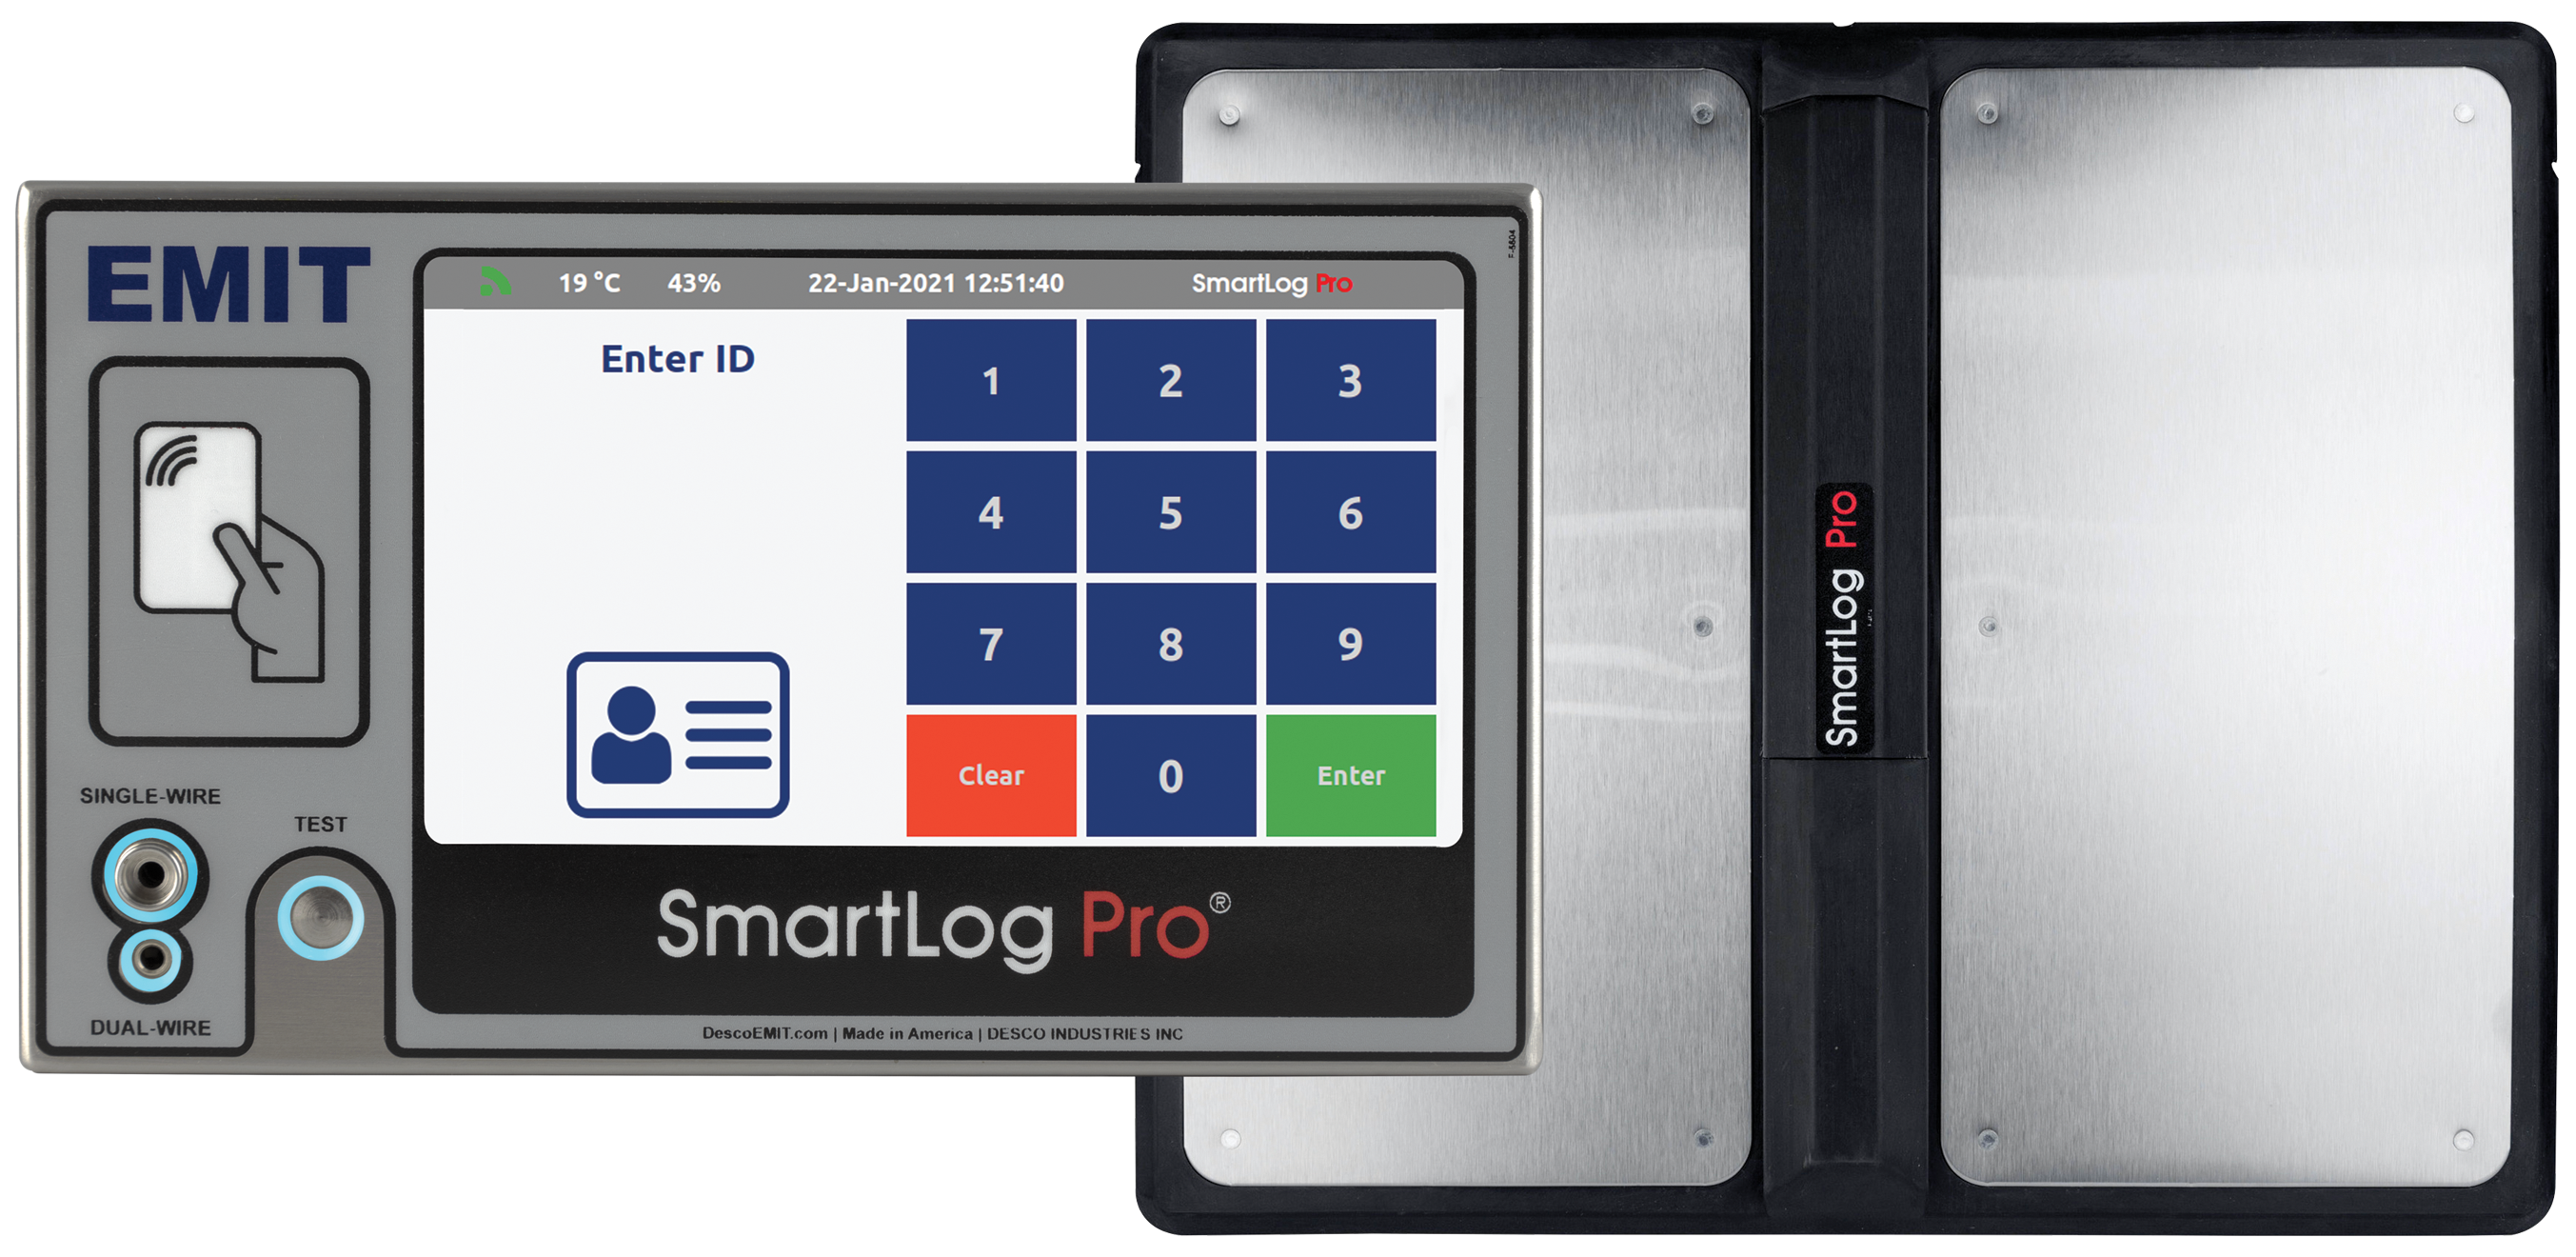
\includegraphics[width=\textwidth]{pics/SAL4_06.png}
    \caption{SmartLog Pro 2 \cite{SmartLogPro2}.}
    \label{fig:smartlog_pro2}
\end{subfigure}

\caption{Sistemas de control ESD avanzados.}
\label{fig:sistemas_esd_avanzados}
\end{figure}

\section{Comparación técnica de alternativas}

A partir de la revisión de literatura, normativas y soluciones comerciales disponibles, se
identifican diferentes niveles de implementación para sistemas de verificación y control
ESD. Estos niveles van desde probadores básicos de pulseras antiestáticas hasta estaciones
industriales avanzadas con identificación de usuario, control de acceso y generación de
reportes. Por esta razón, además de comparar los costos de las soluciones, resulta
necesario realizar una comparación técnica que permita justificar la arquitectura
seleccionada para el prototipo propuesto. En este sentido, se consideran cinco alternativas principales:

\begin{itemize}
    \item \textbf{Probador comercial básico de pulsera antiestática:} corresponde a
    equipos simples utilizados para verificar el estado de una pulsera antiestática. Su
    principal ventaja es el bajo costo y la facilidad de uso; sin embargo, normalmente no
    incorporan identificación de usuario, almacenamiento de datos ni generación de
    reportes \cite{Desco_19240}.

    \item \textbf{Probador comercial de pulsera y calzado ESD:} corresponde a equipos
    capaces de verificar tanto pulseras antiestáticas como sistemas de calzado ESD. Estos
    equipos amplían el alcance de la verificación, pero usualmente mantienen una operación
    local basada en indicaciones visuales de aprobación o rechazo \cite{teknind_dual_esd_tester}.

    \item \textbf{Probador comercial con identificación y control de acceso:} corresponde
    a soluciones que incorporan verificación ESD y algún mecanismo de identificación o
    habilitación de acceso. Este tipo de sistema permite controlar el ingreso a un área o
    estación de trabajo, pero puede requerir accesorios adicionales, configuración
    específica o integración con infraestructura externa \cite{SCS_770758}.

    \item \textbf{Estación comercial avanzada de control ESD:} corresponde a sistemas
    industriales con funciones integradas de verificación de pulsera y calzado,
    identificación de usuario, registro de eventos, generación de reportes, comunicación
    en red, control de acceso e interfaz de usuario. Estas soluciones ofrecen un alto nivel
    de madurez industrial, aunque su costo suele ser elevado y su personalización depende
    de las opciones disponibles por el fabricante \cite{SmartLogPro2}.

    \item \textbf{Prototipo integrado propuesto:} corresponde a la alternativa desarrollada
    en este proyecto. Su arquitectura utiliza un probador comercial de pulseras
    antiestáticas como base de verificación ESD, e integra identificación de usuario,
    monitoreo ambiental, interfaz gráfica táctil, almacenamiento local y generación de
    reportes. Esta alternativa busca cubrir las funciones necesarias para mejorar la
    trazabilidad de las pruebas ESD en un entorno de laboratorio, manteniendo una
    estructura modular, accesible y personalizable.
\end{itemize}

La Tabla~\ref{tab:comparacion_tecnica_alternativas} resume la comparación técnica entre
las alternativas identificadas.

\begin{table}[H]
\centering
\footnotesize
\caption{Comparación técnica entre alternativas de control ESD.}
\label{tab:comparacion_tecnica_alternativas}
\renewcommand{\arraystretch}{1.25}
\begin{tabular}{p{3.3cm}
>{\centering\arraybackslash}p{1.7cm}
>{\centering\arraybackslash}p{1.9cm}
>{\centering\arraybackslash}p{1.9cm}
>{\centering\arraybackslash}p{1.9cm}
>{\centering\arraybackslash}p{1.9cm}}
\toprule
\textbf{Característica} &
\textbf{Desco 19240} &
\textbf{SCS 770758} &
\textbf{PGT130.\newline DT} &
\textbf{SmartLog Pro 2} &
\textbf{Prototipo} \\
\midrule
Verificación de pulsera antiestática & Sí & Sí & Sí & Sí & Sí \\
Verificación de calzado ESD & No & Sí & Sí & Sí & No \\
Identificación de usuario & No & No & Sí & Sí & Sí \\
Almacenamiento de registros & No & No & Sí & Sí & Sí \\
Generación de reportes & No & No & Sí & Sí & Sí \\
Control de acceso & No & Sí & Sí & Sí & No \\
Interfaz gráfica de usuario & No & No & Limitada & Sí & Sí \\
Monitoreo ambiental & No & No & Sí & Sí & Sí \\
Personalización del sistema & Baja & Baja & Media & Media & Alta \\
Dependencia de infraestructura externa & Baja & Baja & Media & Media & Baja \\
Costo relativo & Bajo & Medio & Alto & Alto & Bajo/medio \\
Madurez industrial & Alta & Alta & Alta & Alta & Académica \\
\bottomrule
\end{tabular}
\end{table}

A partir de la comparación anterior, se observa que los probadores comerciales básicos son
adecuados para verificar el estado de una pulsera antiestática, pero no resuelven por sí
solos el problema de trazabilidad, ya que no identifican al usuario ni almacenan registros
históricos. Los probadores de pulsera y calzado amplían la cobertura de verificación ESD,
pero en sus versiones básicas continúan orientados principalmente a una indicación local
de aprobación o rechazo.

Las soluciones comerciales con identificación, control de acceso y reportes representan la
alternativa más completa desde el punto de vista industrial. Sin embargo, su costo elevado,
su dependencia de infraestructura externa y su menor flexibilidad de modificación pueden
hacerlas menos convenientes cuando se busca una solución de bajo costo y adaptable para
un entorno de laboratorio.

En este contexto, el prototipo propuesto se plantea como una alternativa intermedia entre
un probador básico y una estación comercial avanzada. El uso de un probador comercial
como subsistema de verificación reduce el riesgo técnico asociado a la medición de
resistencia cuerpo--tierra, mientras que la integración de identificación, interfaz gráfica,
monitoreo ambiental, almacenamiento local y reportes permite cubrir las funciones
principales requeridas para mejorar la trazabilidad de las pruebas ESD.

\section{Limitaciones de las soluciones existentes}

A partir del análisis del estado del arte, se observa que existen trabajos relacionados con
monitoreo de puesta a tierra, medición de carga electrostática y automatización de pruebas
ante ESD. Sin embargo, no se identifican propuestas orientadas específicamente a una
estación de control ESD de bajo costo que integre verificación de pulseras antiestáticas,
identificación de usuario, almacenamiento local de registros, reportes e interfaz gráfica
en un mismo sistema.

Adicionalmente, no se identifican circuitos integrados \textit{front-end} diseñados de forma
específica para la medición de resistencia cuerpo--tierra en sistemas de control ESD. Por
ello, las alternativas disponibles requieren el uso de probadores comerciales, circuitos de
medición de precisión o instrumentación especializada. En el caso de las soluciones
industriales comerciales, las opciones más cercanas al alcance del proyecto presentan
costos elevados, arquitecturas cerradas y una capacidad de personalización limitada por
las funciones ofrecidas por el fabricante.

Estas limitaciones justifican el desarrollo de un prototipo integrado de bajo costo,
orientado a mejorar la trazabilidad de las pruebas ESD en un entorno de laboratorio. La
solución propuesta no pretende sustituir estaciones industriales certificadas, sino ofrecer
una arquitectura modular y adaptable que permita validar las funciones principales de
identificación, verificación, almacenamiento y reporte requeridas para el caso de estudio.
